\documentclass[12pt]{beamer}
\usecolortheme{ietf93color}

\mode<presentation>
\title{IS-IS Dst/Src Routing}
\subtitle{%
  \href{https://datatracker.ietf.org/doc/draft-baker-ipv6-isis-dst-src-routing/}{draft-baker-ipv6-isis-dst-src-routing-03}
}
\author{%
\href{mailto:fred@cisco.com}{Fred Baker $\cdot$ fred@cisco.com}\\%
\underline{\href{mailto:david@opensourcerouting.org}{David Lamparter $\cdot$ david@opensourcerouting.org}}%
}
\date{IETF 93, Prague, July 2015}
\begin{document}

\begin{frame}
  \titlepage
\end{frame}

\begin{frame}
  \frametitle{Context}
  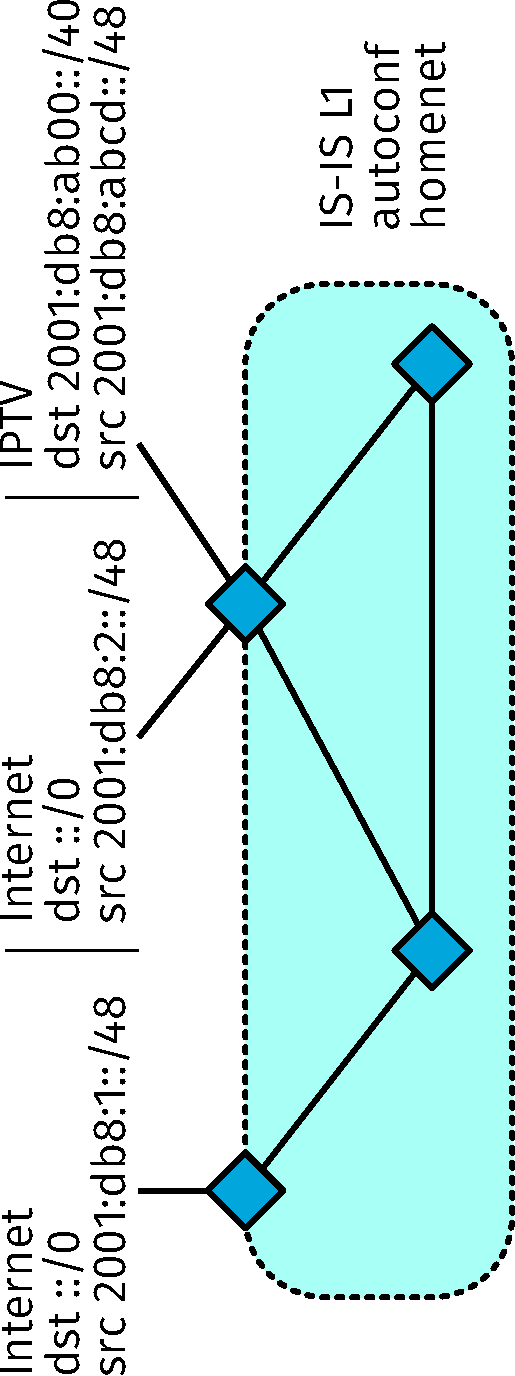
\includegraphics[scale=0.45,angle=-90]{intro_topo.pdf}%
  \vspace{5mm}
  $\Rightarrow$ ensuring correct exit taken based on packet source address
\end{frame}

\begin{frame}
  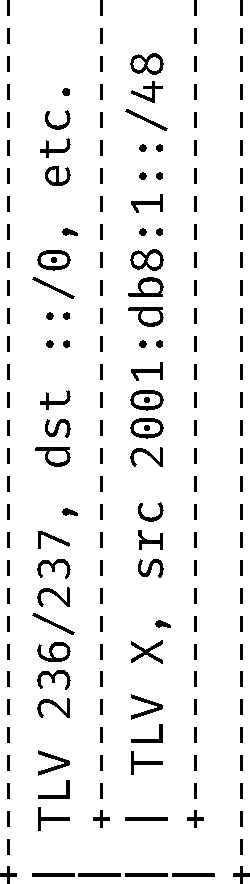
\includegraphics[scale=0.45,angle=-90]{isis_dstsrc_tlv.pdf}%
  \vspace{6mm}
  \begin{itemize}
    \item sticking the source prefix in is straightforward
    \item implemented, tested, demo'd @ IETF 90
    \item open source: \url{https://git-us.netdef.org/projects/OSR/repos/openwrt-isis-hnet}
  \end{itemize}
\end{frame}

\begin{frame}
  \frametitle{Interop / Compatibility}
  \begin{itemize}
    \item naively mixing dst-src routers and non-dst-src routers leads to persistent loops
    \item might be out of scope for homenet
    \item certainly in scope for SMB \& Campus applications
  \end{itemize}
  \vspace{10mm}
  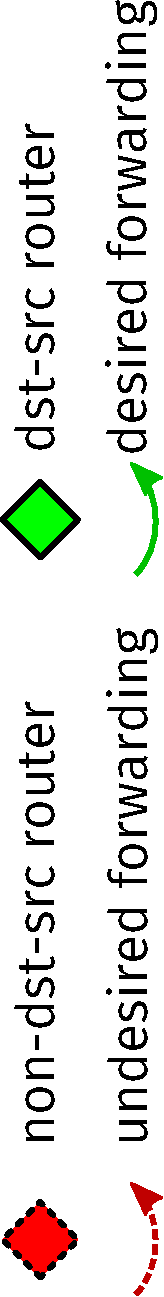
\includegraphics[scale=0.45,angle=-90]{isis_loop_legend.pdf}%
\end{frame}

\begin{frame}
  \frametitle{Loop cases}
  \begin{center}
    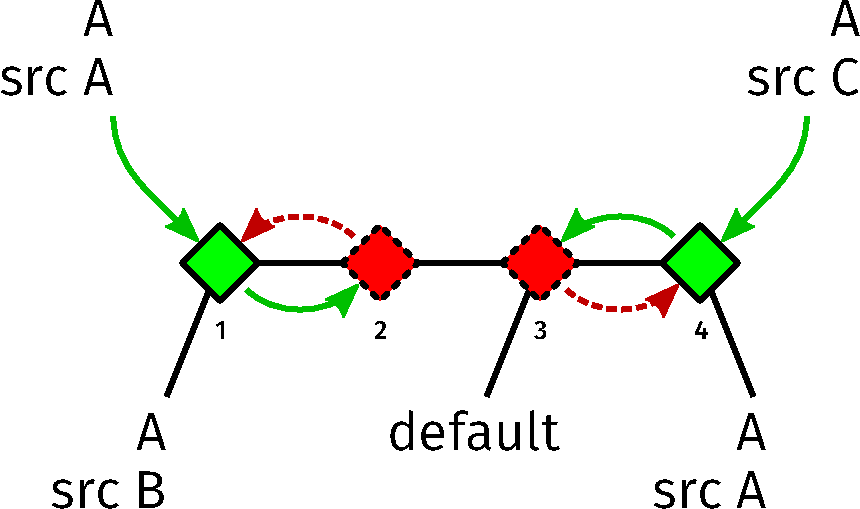
\includegraphics[scale=0.55,angle=0]{isis_93_loop_base.pdf}%
  \end{center}
\end{frame}

\begin{frame}
  \frametitle{Using MT as separation mechanism}
  To fix these scenarios, we need:
  \begin{itemize}
    \item to fix loop \#1: capability indication
    \item to fix loop \#2: hiding reachabilities from ``old'' systems
  \end{itemize}
  \vspace{5mm}
  MT provides both:
  \begin{itemize}
    \item participation in separate topology is capability indication
    \item TLVs in separate topology are invisible to non-participants
  \end{itemize}
\end{frame}

\begin{frame}
  \frametitle{Loop cases}
  \begin{center}
    \includegraphics<1>[scale=0.55,angle=0]{isis_93_loop_base.pdf}%
    \includegraphics<2>[scale=0.55,angle=0]{isis_93_loop_mt1.pdf}%
    \includegraphics<3>[scale=0.55,angle=0]{isis_93_loop_mt2.pdf}%
  \end{center}
  \begin{itemize}
    \item<2-3> \only<2>{A/A hidden from router \#3 $\Rightarrow$ default route works}
               \only<3>{connecting MT islands allows router \#1 to reach A/A}
    \item<2> router \#1 detects non-reachability of A/A
  \end{itemize}
\end{frame}

\begin{frame}
  \frametitle{Route installation}
  \begin{center}
    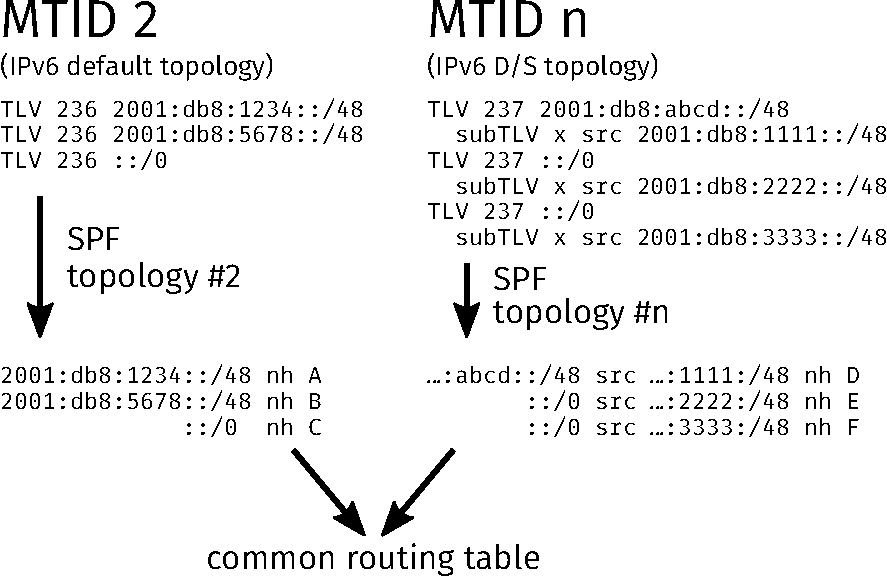
\includegraphics[scale=0.65,angle=0]{isis_93_mtmerge.pdf}%
  \end{center}
\end{frame}

\begin{frame}
  \frametitle{Further path?}
  \begin{itemize}
    \item need to clear topic and proceed
    \item code is running (w/o interop)
  \end{itemize}
\end{frame}

\end{document}
